\section{Simulation Analysis}

\label{sec:simulation}
We ran a simulation of the circuit using {\it Ngspice} with the provided OP-AMP model, thus obtaining the following results, for the frequency analysis of the circuit. 


\begin{figure}[!htb]
     \begin{subfigure}[b]{0.48\textwidth}
         \centering
         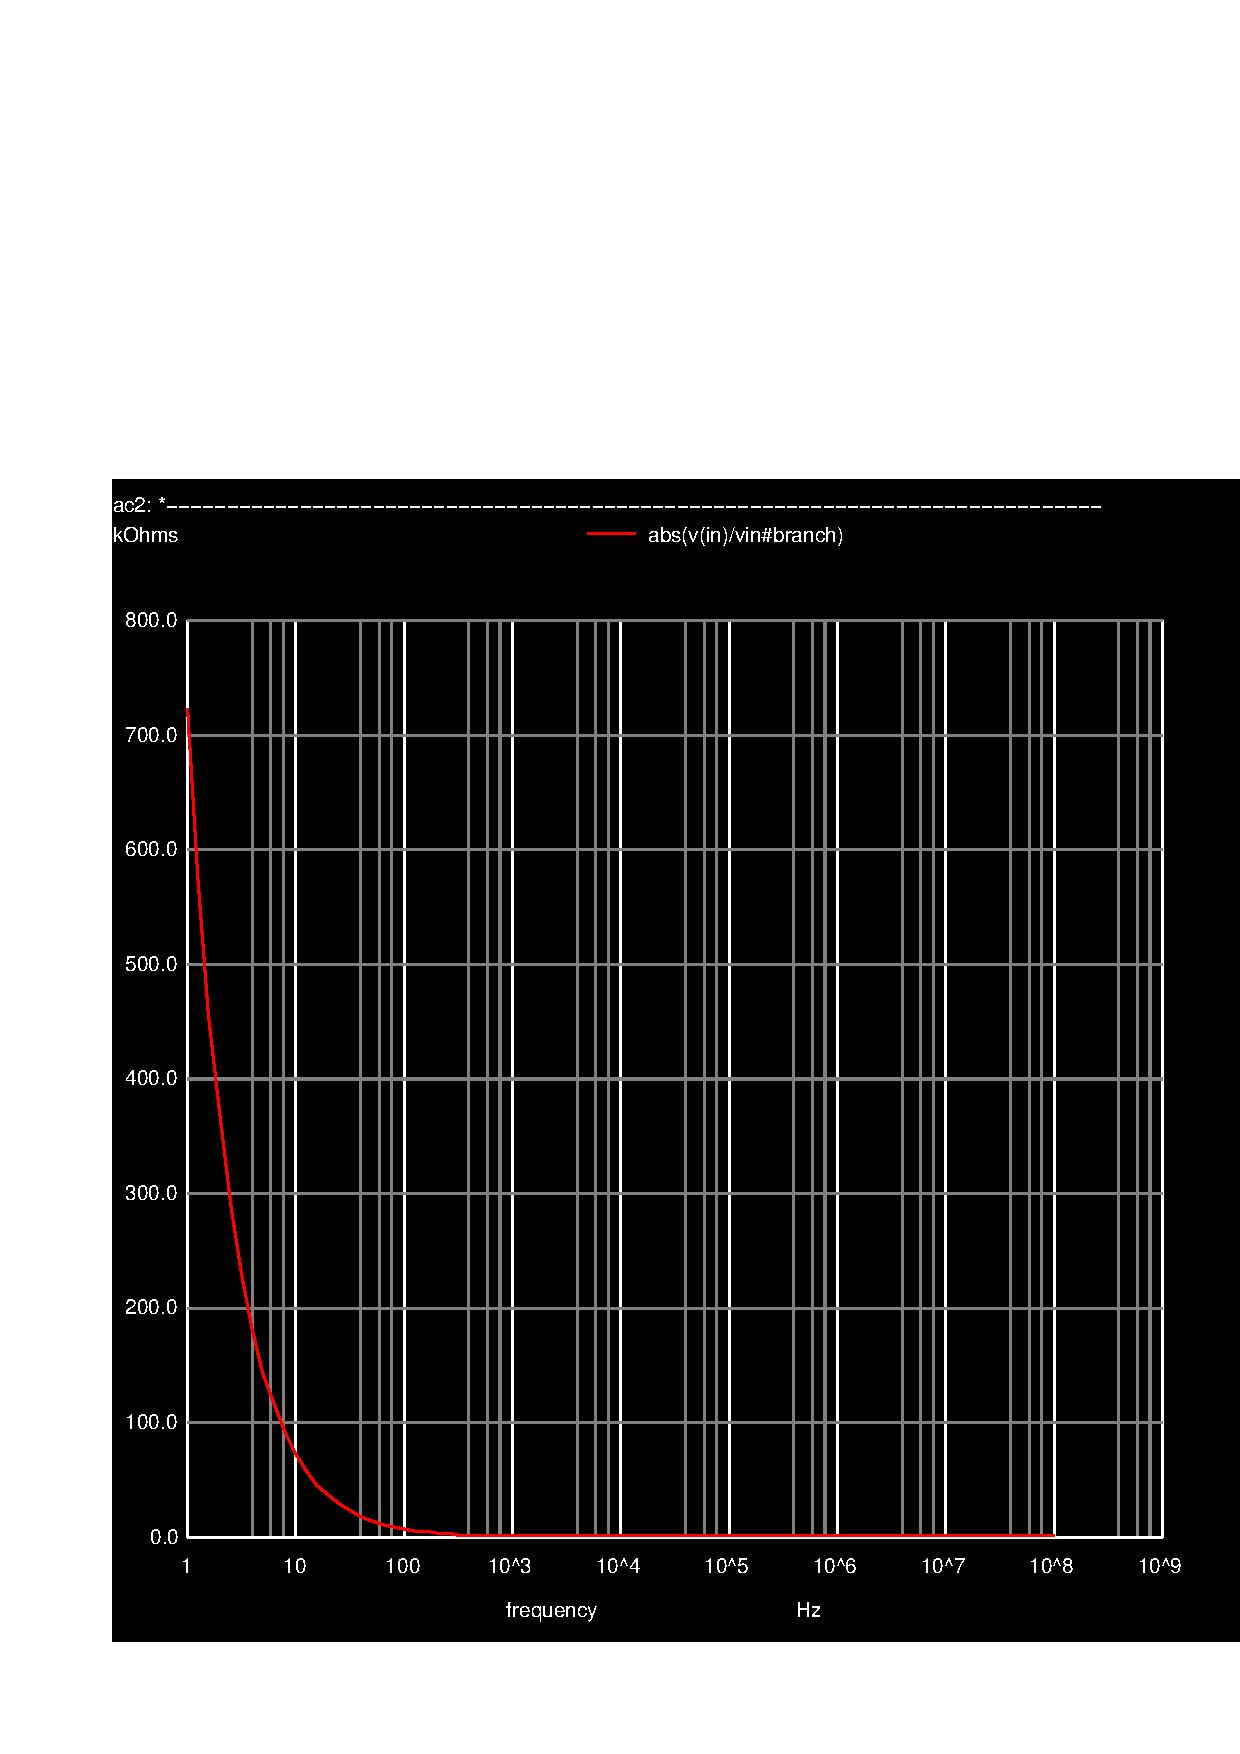
\includegraphics[width=\textwidth]{../sim/1/inputimpedance.pdf}
         \caption{Input impedance of the circuit (kOhm)}
     \end{subfigure}
     \hfill
     \begin{subfigure}[b]{0.48\textwidth}
         \centering
         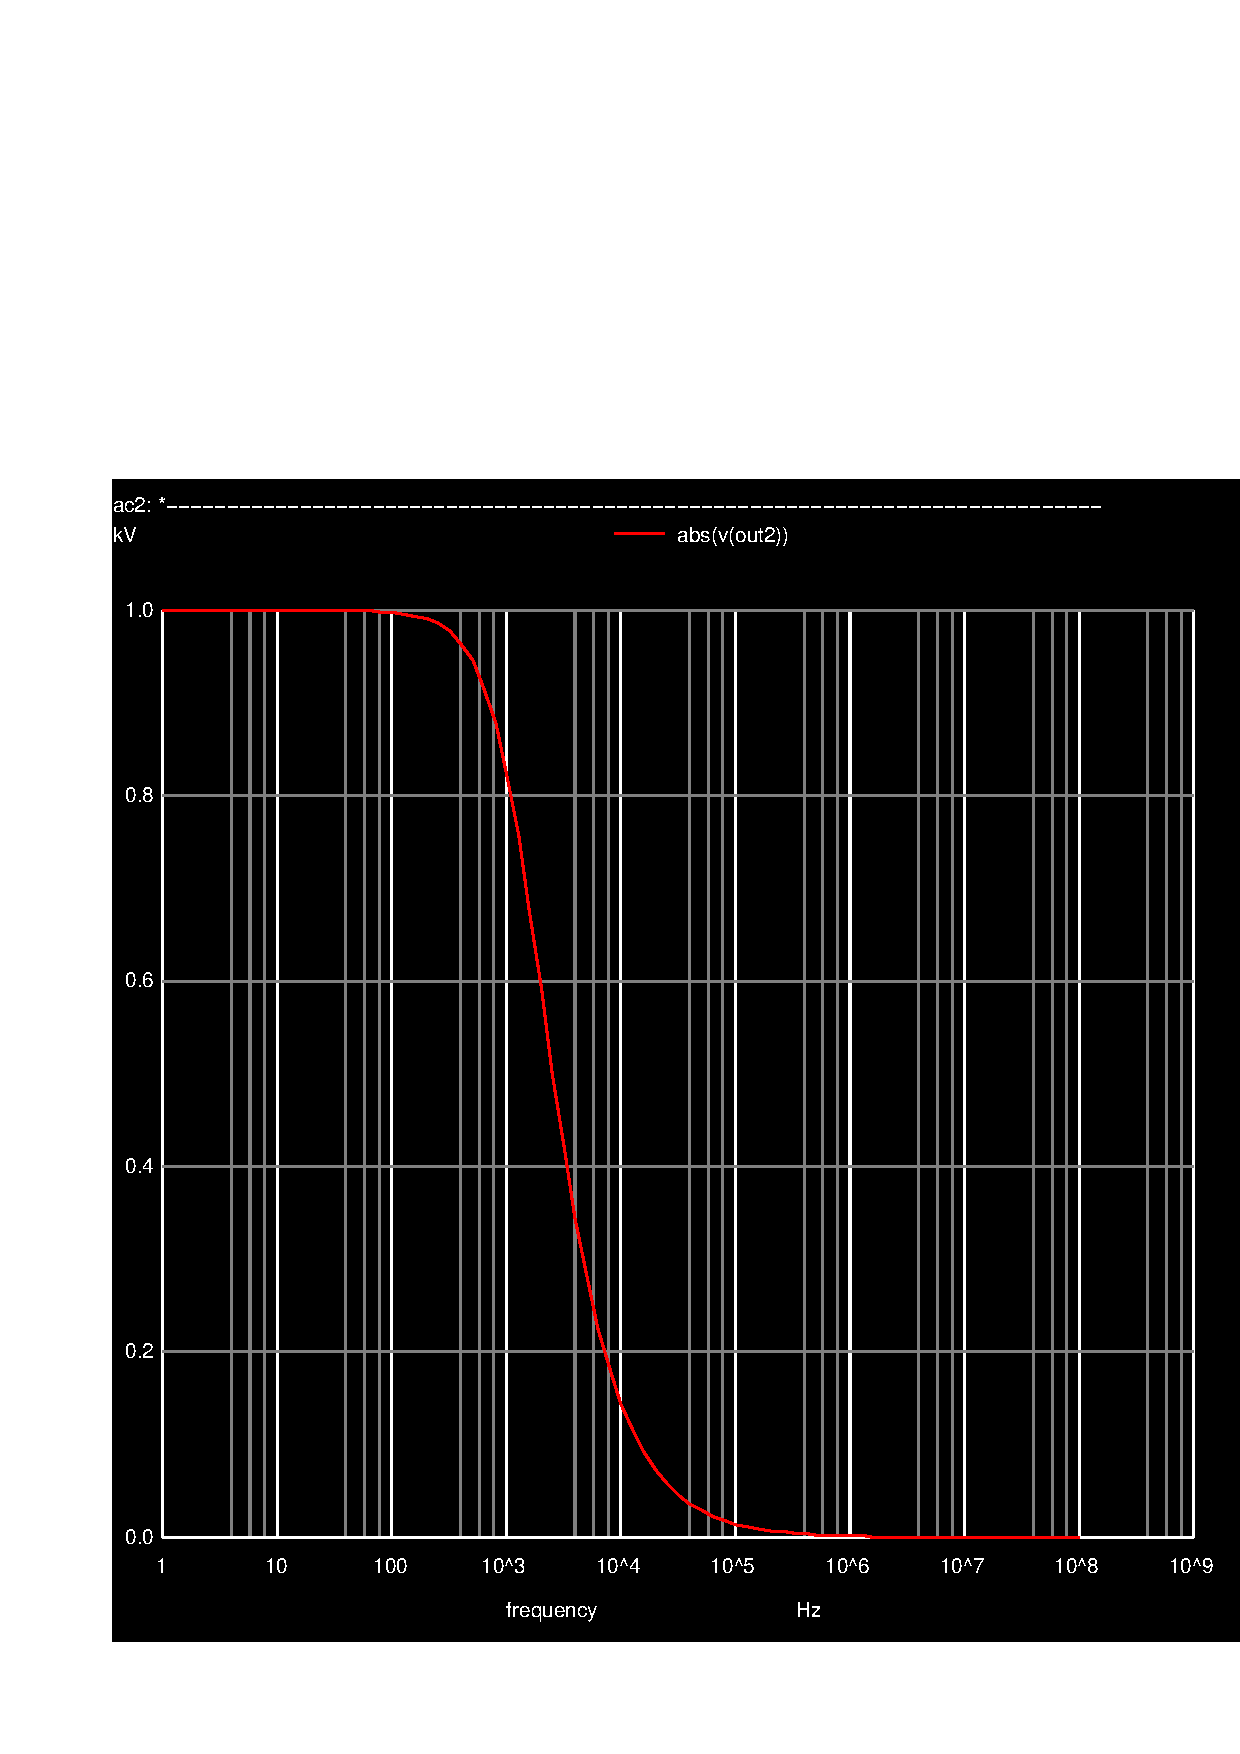
\includegraphics[width=\textwidth]{../sim/2/outputimpedance.pdf}
         \caption{Output impedance of the circuit (kOhm)}
         \label{fig:five over x}
     \end{subfigure}
        \label{fig:two graphs}
\end{figure}


\begin{figure}[!htb]
     \begin{subfigure}[b]{0.48\textwidth}
         \centering
         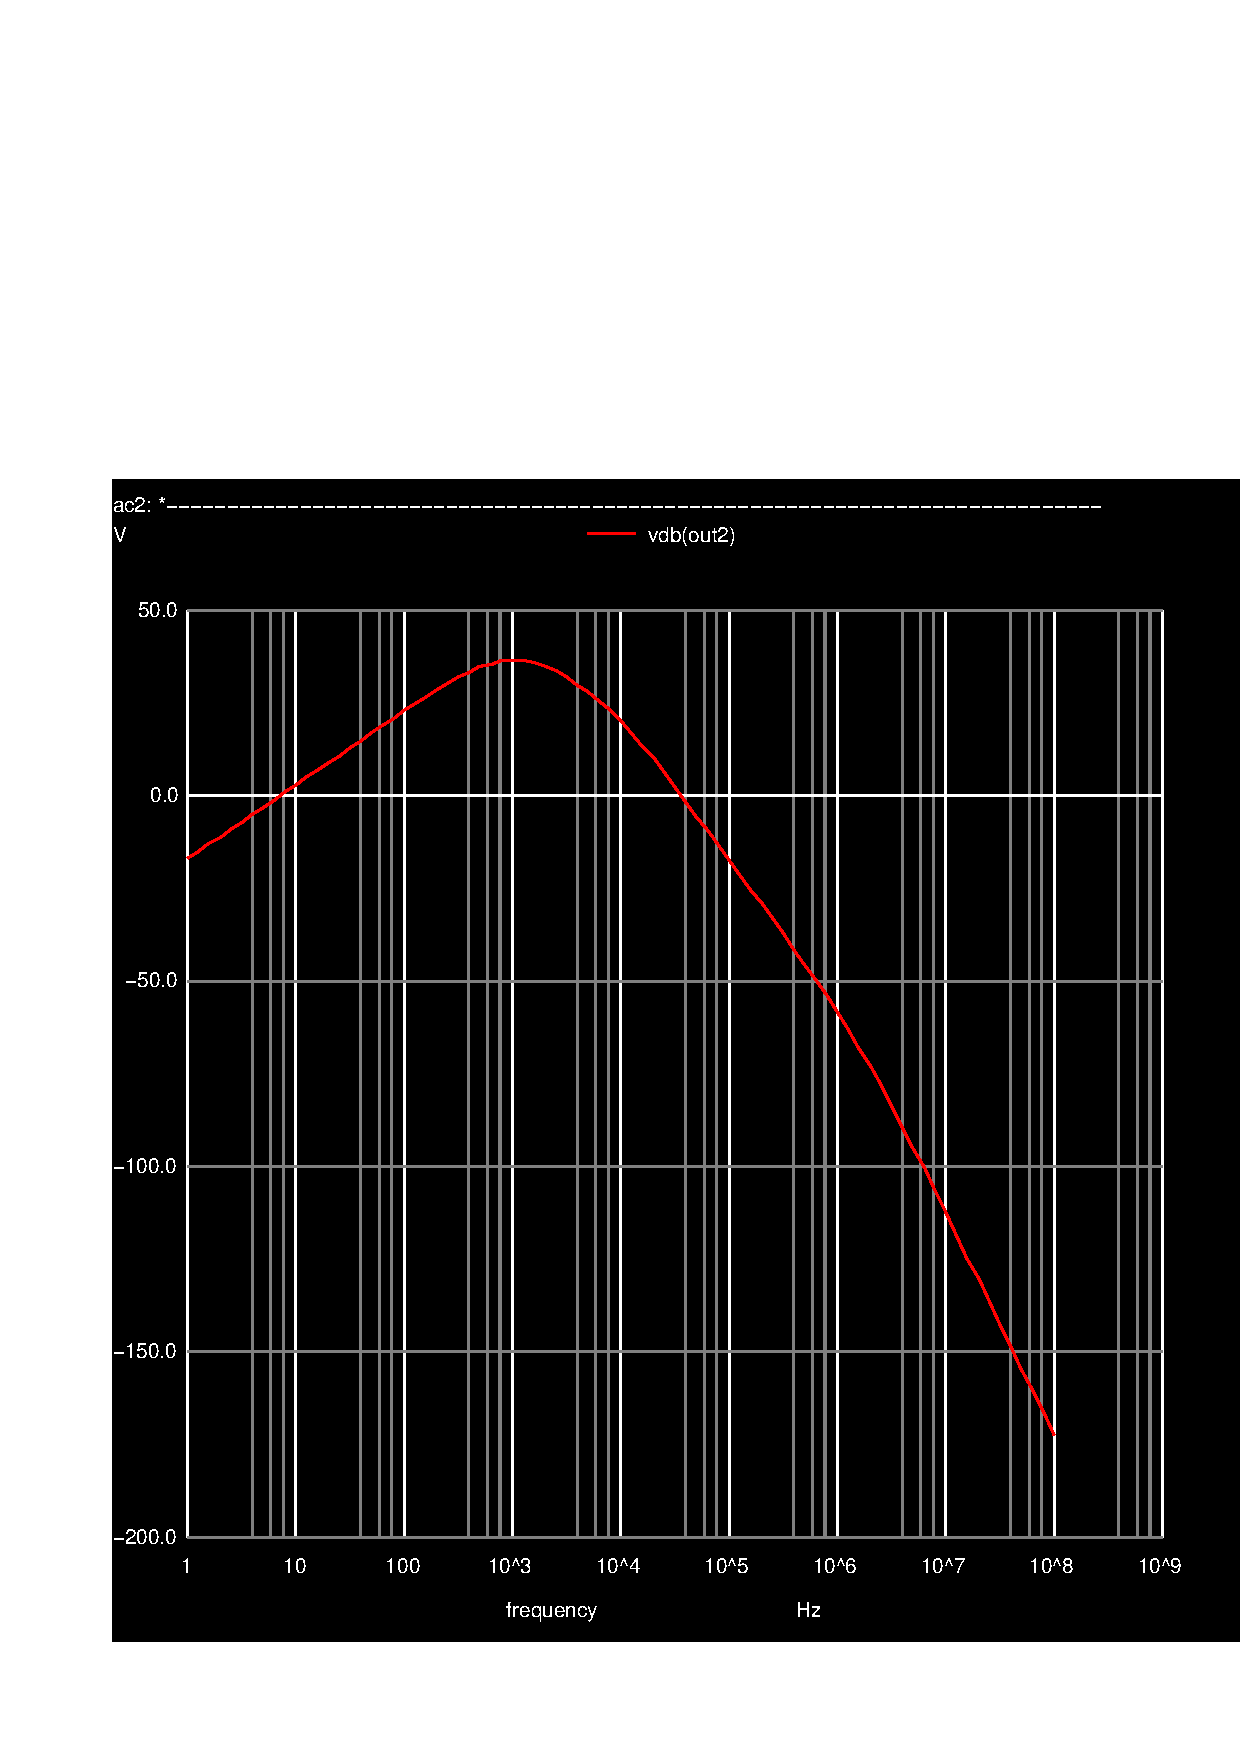
\includegraphics[width=\textwidth]{../sim/1/vo1f.pdf}
         \caption{\textit{Ngspice's} output voltage gain}
     \end{subfigure}
     \hfill
     \begin{subfigure}[b]{0.65\textwidth}
         \centering
         \includegraphics[width=\textwidth]{../mat/Gain.png}
         \caption{Theoretical analysis' output voltage gain}
         \label{fig:five over x}
     \end{subfigure}
     \label{fig:two graphs}
\end{figure}

The input impendence is very high for low frequencies, as expected, and seems to diminuish progressivly for higher frequencies, once again as expected given the frequency dependent behaviour of the capacitor. We also see that for $f \to \infty $ the input impedence appears to vanish, which is a clear deviation from the theoretical model, which considers it to be infinite for all frequencies. 
As for the ouput impendence, the results obtained show the predicted behaviour. The total output impedence is approximatly just due to the capacitor resistor association, thus leading to a similar behaviour. It should be noted that the high ouput impedence values are not ideal to connect to any load, as there can be significant voltage loss.
The output voltage gain plot shows a very narrow passband centered at approximatly 1kHz. Hence, the circuit effectivly acts as a passband filter, althought one with very little bandwith. We did not consider this to be a problem as on of the requirements was a central frequency, $f = \sqrt{f_{lower}f_{upper}}$ of\footnote{upper and lower cut-off frequencies were calculated as the frequencies for wich the gain was less 3dB than at it's maximum.} 1kHz. The specificity of the value requested led us to think the filter was very directed for 1kHz and neighbouring frequencies. 
Furthermore, the gain plot obtained with the theoretical analysis is very coherent with the simulation. Both show similar form, peaking at around 1kHz, correponding to a gain of about 35-40 dB. The significant diferences occur for frequencies greater than 0.1MHz, for which \textit{ngspice's} reveals a much quicker decreace in gain, eventually reaching -150dB where spice never reaches bellow -100dB. This divergence may be rooted in the aformentioned input impedence which diminuishes significantly.  
What is more, we calculated the gain, input and output impendences at the central frequency.
  	 
\begin{table}[h]
  \centering
  \begin{tabular}{|l|r|}
    \hline    
    {\bf Name} & {\bf Value [A or V]} \\ \hline
    f & 1.004690e+03\\ \hline
gain & 3.652900e+01\\ \hline
z & 1.519501e+03\\ \hline

    f & 1.004690e+03\\ \hline
gain & 3.652900e+01\\ \hline
z & 1.519501e+03\\ \hline

  \end{tabular}
  \caption{$f$ denotes the central frequency, Z the input impedence and mag(z) the output impedence.}
\end{table}

Once again, the value for the gain is in agreement with the theoretical analysis.  

XXXXX Hence we obtainned, a merit figure of $2,1 \times 10^7$.




	



